\documentclass[xcolor=table]{beamer}
\usepackage[english,russian]{babel}
\usepackage[utf8]{inputenc}


\newcommand{\setR}{\mathbb{R}}
\newcommand{\setN}{\mathbb{N}}
\newcommand{\setRn}{\mathbb{R}^n}
\newcommand{\setN}{\mathbb{N}}
\newcommand{\manX}{\mathcal{X}}
\newcommand{\bp}{{\bf P}}
\newcommand{\bs}{{\bf s}}
\newcommand{\bS}{{\bf S}}
\newcommand{\bw}{{\bf W}}
\newcommand{\bx}{{\bf X}}
\newcommand{\bc}{{\bf C}}
\newcommand{\bd}{{\bf D}}
\newcommand{\bsm}{{\bf s}}
\newcommand{\bl}{{\bf L}}
\newcommand{\by}{{\bf Y}}
\newcommand{\ba}{{\bf A}}
\newcommand{\manM}{\mathcal{M}}
\newcommand{\manH}{\mathcal{H}}
\newcommand{\spn}{S^+(n,p)}

\newcommand{\condset}[2]{\braces{\, #1 \mid #2 \,}}
\newcommand{\walls}[1]{\left | #1 \right |} 
\newcommand{\norm}[2]{\left{||}#1\right{||}_{#2}} 
\newcommand{\set}[1]{\left\{ #1 \right\}}
\newcommand{\inprod}[3]{\left < #1,#2\right >_#3}

\usepackage{lmodern}    \usepackage[labelformat=empty,font=scriptsize,skip=0pt,justification=justified,singlelinecheck=false]{caption}

%remove the icon
\setbeamertemplate{bibliography item}{}

%remove line breaks
\setbeamertemplate{bibliography entry title}{}
\setbeamertemplate{bibliography entry location}{}
\setbeamertemplate{bibliography entry note}{}

\usepackage[square,numbers]{natbib}
\newcounter{totfigures}
\newcounter{tottables}
\newcounter{totreferences}
\makeatletter
\renewcommand{\@dotsep}{2}
\newcommand{\l@likechapter}[2]{{\bfseries\@dottedtocline{0}{0pt}{0pt}{#1}{#2}}}
\AtEndDocument{%
  \addtocounter{totfigures}{\value{figure}}%
  \addtocounter{tottables}{\value{table}}%
  \immediate\write\@mainaux{%
    \string\gdef\string\totfig{\number\value{totfigures}}%
    \string\gdef\string\tottab{\number\value{tottables}}%
    \string\gdef\string\totref{\number\value{totreferences}}%
  }%
}
\makeatother
\pretocmd{\chapter}{\addtocounter{totfigures}{\value{figure}}}{}{}
\pretocmd{\chapter}{\addtocounter{tottables}{\value{table}}}{}{}
\pretocmd{\bibitem}{\addtocounter{totreferences}{1}}{}{}
\newcommand{\likechapterheading}[1]{
	\begin{center}
	\textbf{\MakeUppercase{#1}}
	\end{center}
	\empline}
\newcommand{\likechapter}[1]{	
	\phantomsection
	\likechapterheading{#1}	
	\addcontentsline{toc}{likechapter}{\texorpdfstring{\MakeUppercase{#1}}{#1}}}
\newcommand{\empline}{\mbox{}\newline}
\renewcommand{\bibnumfmt}[1]{[#1]\hfill}
\renewcommand{\bibsection}{\likechapter{Список литературы}}
\setlength{\bibsep}{0pt}

\newcommand{\append}[1]{
	\clearpage
	\stepcounter{chapter}	
	\paragraph{\MakeUppercase{#1}}
	\empline
	\addcontentsline{toc}{likechapter}{\texorpdfstring{\chaptertitlename~\Asbuk{chapter}\;#1}}{\chaptertitlename~\Asbuk{chapter}:~#1}}
	
	
\usetheme{Darmstadt}
\begin{document}
\title[]{Применение геометрии многообразия симметричных положительно полуопределенных матриц в анализе данных головного мозга}  
\author[Дарья Беляева]{Беляева Дарья, гр. 177 \\ Научный руководитель: Бурнаев Е.В., к.ф.-м.н}
\institute{МФТИ(ГУ) \\ Факультет управления и прикладной математики \\ Кафедра проблем передачи информации и анализа данных}
\vfill
\date{Москва, 2017} 

\frame[plain]{\titlepage} 


% \AtBeginSection[]
% {
%   \begin{frame}
%   \frametitle{Содержание}
%   \tableofcontents[currentsection]
%   \end{frame}
% }

%\frame[plain]{\frametitle{Содержание}\tableofcontents}

\section[]{Постановка задачи}
    \begin{frame}
    \frametitle{Постановка задачи}
    \begin{itemize}
        \item Рассмотреть существующие подходы к классификации СПО и СППО матриц
        \item Предложить эффективный алгоритм классификации СППО матриц
    \end{itemize}
    \end{frame}
    
\section[Существующие подходы]{Существующие подходы}
    \subsection[Классификация в касательном пространстве]{Классификация в касательном пространстве}
    \begin{frame}
    \frametitle{Классификация в касательном пространстве}
    \framesubtitle{Существующие подходы}
    В пространстве СПО матриц возможно выполнить проекцию на касательное пространство:
    \begin{figure}
        \centering
        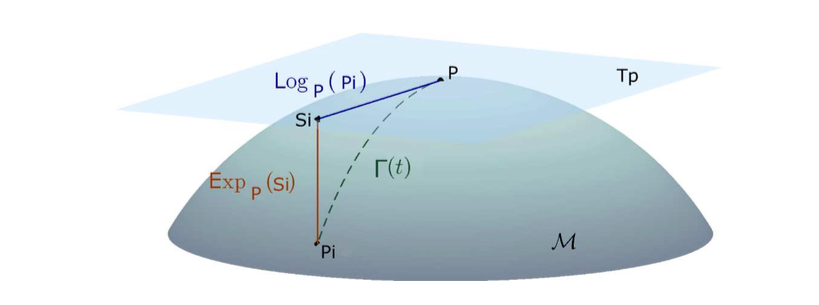
\includegraphics[width=\textwidth]{img/tangent_space}
        \caption{Касательное пространство в точке $\bp$, $\bS_i$ - касательный вектор к точке $\bp$ и $\Gamma_i(t)$ - геодезическая между $\bp$ и $\bp_i$}
    \end{figure}
    Подход использован, например, в \cite{barachant2012multiclass}, \cite{barachant2013classification}
    \end{frame}
    
    \subsection[Классификация с помощью ядерных алгоритмов]{Классификация с помощью ядерных алгоритмов}
    \begin{frame}
    \frametitle{Классификация с помощью ядерных алгоритмов}
    \framesubtitle{Существующие подходы}
    \begin{block}{Гауссовское ядро}
    \begin{equation}
        \label{gaussian_kernel}
        K(x_i, x_j) = exp\Big(\frac{||x_i - x_j||^2}{2\sigma^2}\Big) 
    \end{equation}
    \end{block}
    \begin{block}{Ядро на основе расстояний $\delta_{spd}$}
    Пусть $\bs_i, \bs_j \in S(n)$
    \begin{equation}
        \label{kernel}
        K_{spd}(\bs_i, \bs_j) = exp(-\gamma \delta_{spd}(\bs_i, \bs_j))
    \end{equation}
    \end{block}
    Подход использован в работах \cite{jayasumana2013kernel}, \cite{dodero2015kernel}
    \end{frame}

\section[Предложенный метод]{Предложенный метод}
\subsection[Предложенные методы]{Предложенные методы}
    \begin{frame}
    \frametitle{Предложенные методы}
    \begin{table}
    \centering
    \resizebox{\textwidth}{!}{
    \begin{tabular}{ll}
    \rowcolor[HTML]{EFEFEF} 
    \hline
    \multicolumn{1}{c}{\cellcolor[HTML]{EFEFEF}Существующий подход} & \multicolumn{1}{c}{\cellcolor[HTML]{EFEFEF}Предложенный подход}                                                                               \\ \hline
    Проекция на касательное пространство                            & \begin{tabular}[c]{@{}l@{}}Снижение размерности Isomap \cite{krivov2016dimensionality} \cite{} \\ на СППО матрицах\end{tabular}                                                       \\ \hline
    Ядерный SVM + $\delta_{spd}$                                    & \begin{tabular}[c]{@{}l@{}}Ядерный SVM + $\delta_{spsd}$:\\ $ K_{spsd}(\bs_i, \bs_j) = exp(-\gamma \delta_{spsd}(\bs_i, \bs_j)) $\end{tabular} \\ \hline
    \end{tabular}}
    \end{table}
    
    \begin{block}{$\delta_{spsd}$ - длина геодезической}
    \begin{equation}\label{spsd_distance}
        \delta_{spsd} = l^2(\gamma_{A \to B}) = ||\Theta||_F^2 + k ||\log R_A^{-1} R_B^2 R_A^{-1}||_F^2
    \end{equation}
    Предложено в \cite{bonnabel2008geometric}
    \end{block}
    \end{frame}
     
    % \subsection[Расстояние в пространстве СППО матриц]{Расстояние в пространстве СППО матриц}
    % \begin{frame}
    % \frametitle{Расстояние в пространстве СППО матриц}
    % $\Theta = diag(\theta_1, \ldots, \theta_p)$ - углы между пространствами. \\
    %  \\
    % $||\log R_A^{-1} R_B^2 R_A^{-1}||_F^2$ - длина геодезической в $S(n)$
    % \begin{block}{$\delta_{spsd}$ - длина геодезической}
    % \begin{equation}\label{spsd_distance}
    %     \delta_{spsd} = l^2(\gamma_{A \to B}) = ||\Theta||_F^2 + k ||\log R_A^{-1} R_B^2 R_A^{-1}||_F^2
    % \end{equation}
    % \end{block}
    % Это измерение было предложено в \cite{bonnabel2009riemannian}
    % \end{frame}
    
      
\section[Данные]{Данные}

    \subsection[МРТ]{Магнитно-резонансная томография}
    \begin{frame}
    \frametitle{Магнитно-резонансная томография}
    \framesubtitle{Методы исследования мозга}
    Современный, более точный неинвазивный метод
    \begin{itemize}
        \item регистрирует электромагнитный отклик атомных ядер
        \item данные воспроизводимы
        \item реализует объемную регистрацию
    \end{itemize}
    Два типа МРТ - диффузионная (структурная) и функциональная
    \end{frame}
    
    \subsection[Коннектомы]{Коннектомы}
    \begin{frame}
    \frametitle{Коннектомы}
    \framesubtitle{Методы исследования мозга}
    Коннектом - представление структурных или функциональных связей мозга в виде взвешенного неориентированного графа.
    \begin{itemize}
        \item вершины - регионы мозга
        \item ребра - структурные (физиологические) либо функциональные связи
    \end{itemize}
    \begin{figure}[h]
    	\centering
    	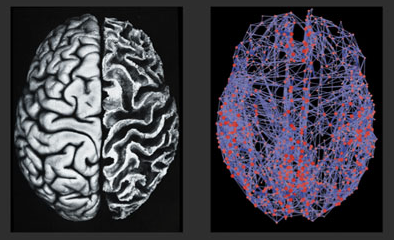
\includegraphics[width=0.7\textwidth]{./img/connectome_pres}
    \end{figure}
    \end{frame}
    
\begin{frame}
    \frametitle{Данные}
    База данных Alzheimer's Disease Neuroimaging Initiative.
    \begin{itemize}
        \item 228 пациентов
        \item 4 класса: NC (61), EMCI (77), LMCI (43), AD (50)
        \item Средний возраст пациентов: 72.9 $\pm$ 7.4 лет
        \item Итоговый коннектом содержит 68 вершин для каждого снимка
    \end{itemize}
    \end{frame}

\section[Эксперименты]{Эксперименты}  

    \subsection[Преобразование данных к СППО матрицам]{Преобразование данных к СППО матрицам}
    \begin{frame}
        \frametitle{}
        \framesubtitle{Эксперименты}
        Коннектом - симметричная не определенная матрица. Применяем преобразование Лапласа \cite{dodero2015kernel}:
        $$\bx_i = \bd_i^{-\frac{1}{2}} (\bd_i - \ba_i) \bd_i^{-\frac{1}{2}},$$
        где $$\bd_i \rvert_{k,k} = \sum_{\substack{l}} \ba_i\rvert_{k,l}$$
    \end{frame}

    \subsection[Сравнительные методы]{Сравнительные методы}
    \begin{frame}
    \frametitle{Сравнительные методы}
    \framesubtitle{Эксперименты}
    \begin{itemize}
        \item Kernel SVM с матрицей $L2$ расстояний между матрицами
        \item Kernel SVM с матрицей логарифмированного евклидового расстояния между регуляризованными матрицами \cite{dodero2015kernel}
    \end{itemize}
    \end{frame}

    \subsection[Результаты]{Результаты}
    \begin{frame}
    \frametitle{Результаты}
    \framesubtitle{Эксперименты}
    \begin{figure}[h!]
    \centering
    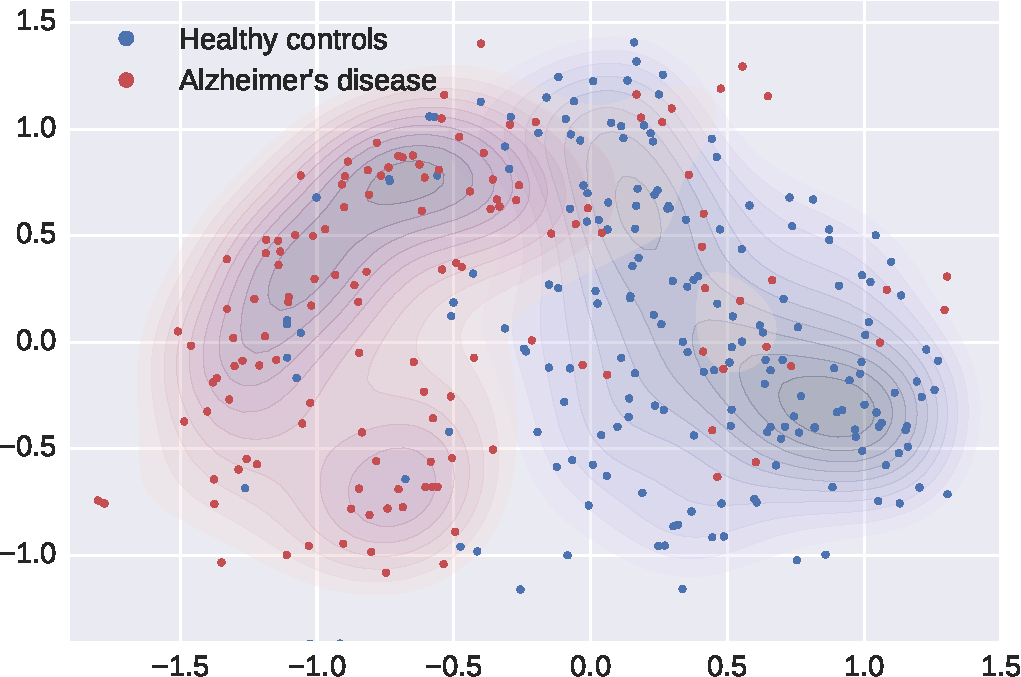
\includegraphics[width=0.8\textwidth]{img/dr.pdf}\label{fig:dr}
    \caption{Данные классов AD и NC, спроецированные на двумерное пространство. Синий и красный цвета обозначают NC и AD группы соответственно.}
    \end{figure}
    \end{frame}


    \begin{frame}
    \frametitle{Результаты}
    \framesubtitle{Эксперименты}
    \begin{table}[h!]
    \centering
    \resizebox{\textwidth}{!}{
    \begin{tabular}{lllll}
    \hline
    \rowcolor[HTML]{EFEFEF} 
    Пара классов & SVM + L2 & SVM + SPD & Isomap $\delta_{spsd}$ & SVM + $\delta_{spsd}$ \\
    \hline
    (AD, NC)     & 77.2 $\pm$ 0.99     & 80 $\pm$ 0.54                           & \cellcolor[HTML]{E1FFCF}81.6 $\pm$ 0.6           & \cellcolor[HTML]{E1FFCF}81.6 $\pm$ 0.7                        \\
    (AD, LMCI)   & 65.5 $\pm$ 1.6      & \cellcolor[HTML]{E1FFCF}68.8 $\pm$ 0.81 & 67.8 $\pm$ 0.6                                   & 68.6 $\pm$ 1.4                                                \\
    (LMCI, EMCI) & 44.7 $\pm$ 2.9      & \cellcolor[HTML]{E1FFCF}47.8 $\pm$ 2.4  & 34.1 $\pm$ 0.59                                  & 44.1 $\pm$ 2.2                                                \\
    (EMCI, NC)   & 50.4 $\pm$ 1.8      & 53.9 $\pm$ 1.6                          & 53.8 $\pm$ 0.12                                  & \cellcolor[HTML]{E1FFCF}{\color[HTML]{000000} 57.1 $\pm$ 1.5}
    \end{tabular}}
    \caption{Сравнительные результаты классификации всех четырех алгоритмов, рассматривавшихся в работе. Цветом выделены лучшие результаты для каждой пары классов. Метрика качества – ROC AUC}
    \end{table}
    \end{frame}
    
    \begin{frame}
    \frametitle{Результаты}
    \framesubtitle{Эксперименты}
    \begin{figure}[h!]
    \centering
    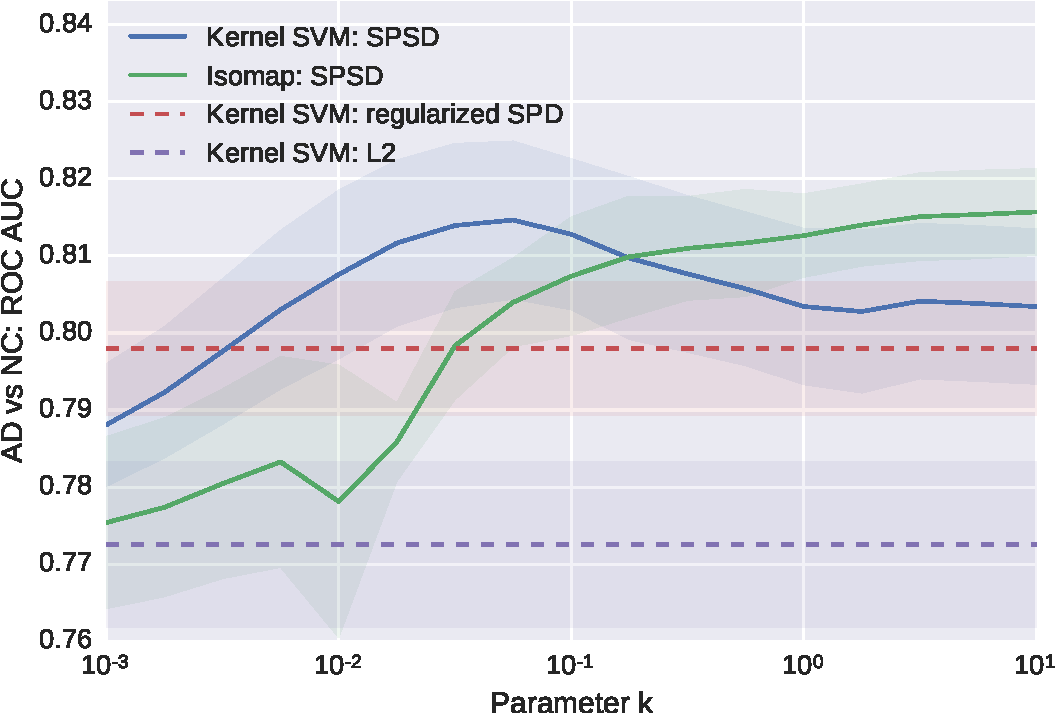
\includegraphics[width=0.8\textwidth]{img/k_dep.pdf}\label{fig:clf_quality}
    \caption{Качество классификации как функция от параметра $k$.}
    \end{figure}
    \end{frame}


\section[Заключение]{Заключение}

\begin{frame}
\frametitle{Заключение}
\begin{block}{}
\begin{itemize}
    \item Рассмотрены подходы к классификации СПО, СППО матриц
    \item Предложен более эффективный алгоритм классификации СППО матриц
\end{itemize}
\end{block}
\end{frame}

\begin{frame}[shrink=50,fragile]
    \frametitle{Список литературы}
    \bibliographystyle{apalike}
    \bibliography{refpres}
\end{frame}

\begin{frame}
    \frametitle{Обозначения}
    \framesubtitle{Математический аппарат}
    
    \begin{itemize}
    	\item $Sym(n) = \condset{\bs \in M(n)}{\bs^T \ = \ \bs}$ пространство всех симметричных матриц в $M(n)$.
    	\item $S(n)$ - множество всех симметричных положительно определенных (СПО) матриц размера $n \times n$.
    	\item $S^+(n, p)$ – множество всех симметричных положительно полуопределенных (СППО) матриц размера $n \times n$ и ранга $p \leq n$.
    	\item $T_p \manM$ - касательное пространство к многообразию $\manM$ в точке $p$.
    	\item $V_{n,p}$ - множество матриц размера $n \times p$ с ортонормальными столбцами: $U^TU=I_p$
    	\item $O(n)$ - ортогональная группа
    \end{itemize}
    
    \end{frame}
    
\end{document}